\chapter{System Analysis and Design}
\section{Introduction}
Systems analysis is a problem solving technique that decomposes a system into its component pieces 
for the purpose of the studying how well those component parts work and interact to accomplish their purpose~\cite{SystemsAnalysisandDesign}.
Systems design is the process of defining the architecture, components, modules, interfaces and data for a system to satisfy specified requirements. 
This chapter explains the modules of read configuration, initialize CA, update state of CA, properties of ES and BCs, save results, quantify and generate images.

\section{Objectives of the system}
The system should read the parameters from a configuration file, initialise CA with ECM, place one CSC in center and start simulation. 
The results should be saved, which should contain BC count, FD in each zone at every simulation step. 
Every ten simulation step entire CA state should be saved.
For results of every ten simulation step there should be hassle free transformation to biological equivalent image.

\section{System design}

The proposed system is a Computational lattice consisting of cancer cell (C), 
ECM site (E) and free space (F). 

\section{Modules design}

  \subsection{Get configuration}
  Get configuration module reads parameter name and the value from configuration file. 
  Parameter types are integer or real. 
  \begin{figure}[H]
	  \centering
	  \fbox{ 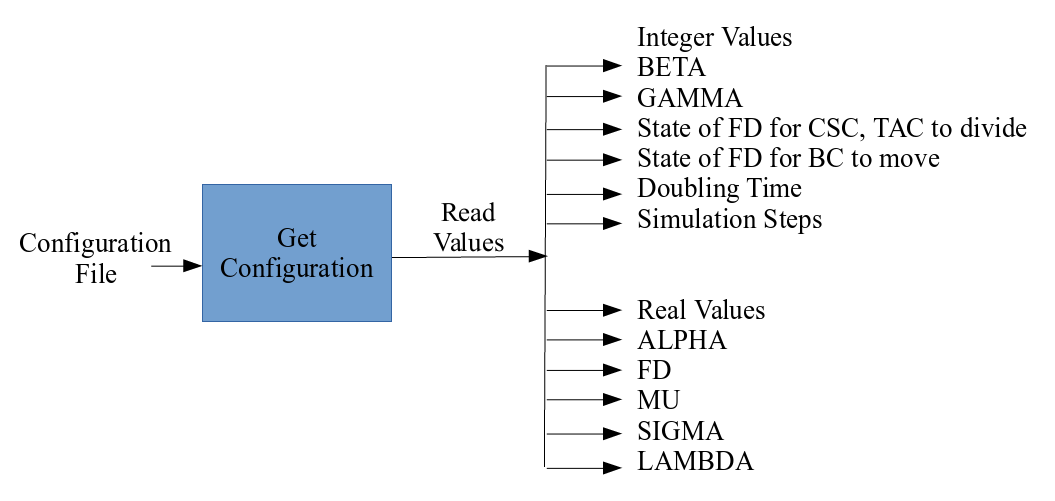
\includegraphics[scale=0.27]{images/GETCONFIGURATION.png} }
	  \caption{Get configuration}
	  \label{GETCONFIGURATION}
  \end{figure}
  \noindent Integer parameters to be read are $\beta$, $\gamma$, state of fiber density for CSC, TAC to divide, state of fiber density for BC to move,
  Doubling Time, Simulation Steps. Real valued parameters to be read are $\alpha$, FD, $\mu$, $\sigma$, $\lambda$.
  Get configuration module then forwards the value to initialization module.

  
  \subsection{Initialization of Cellular Automata}
  
  Initialization module takes input from get configuration module and sets properties of CA, and places one CSC in center, 
  surrounded by ES with FD as fiber density and about $\sigma$ number of ES (Figure \ref{Initialization} and Figure \ref{InitializationFlowChart}).
  It then calls simulation module.
  
      \begin{figure}[H]
	  \centering
	  \fbox{ 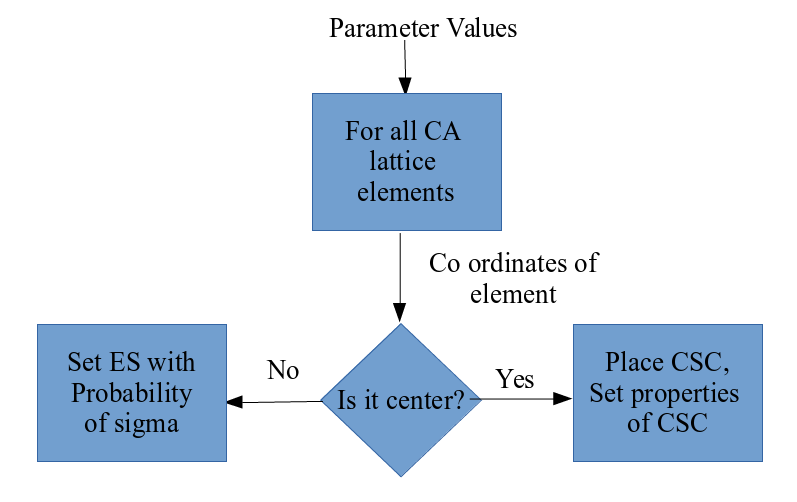
\includegraphics[scale=0.35]{images/InitializationFlowChart.png} }
	  \caption{Flow for initialization of Cellular Automata}	
	  \label{InitializationFlowChart}
  \end{figure}   


    \begin{figure}[H]
	  \centering
	  \fbox{ 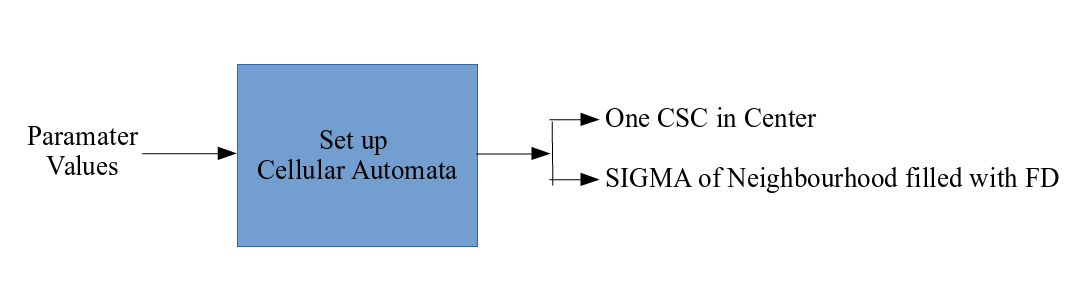
\includegraphics[scale=0.35]{images/Initialization.png} }
	  \caption{Initialization of Cellular Automata}
	  \label{Initialization}
  \end{figure}

  
  

\section{Conclusion}
This chapter explains about different units like read configuration, initialization, update CA, properties of ES and BC, 
quantify results and generate images modules in detail that are used to design the system.


